\chapter{Problem Statement and Motivation}

The entry point to research in this area was asking the question ``How does the software managing critical infrastructure like FREEDM behave when a critical component, the communication infrastructure, is not operating correctly?'' 
Historically, leader elections have had limited applications in critical systems. However, in the smart grid domain, there is a great opportunity to apply leader election algorithms in a directly beneficial way. \cite{LOADBALANCING} presented a simple scheme for performing power distribution and stabilization that relies on formed groups. Algorithms like Zhang, et. al's Incremental Consensus Algorithm \cite{INCREMENTALCONSENSUS}, begin with the assumption that there is a group of nodes who coordinate to distribute power. In a system where 100\% up time is not guaranteed, leader elections are a promising method of establishing these groups.
A strong cyber-physical system should be able to survive and adapt to network outages in both the physical and cyber domains. When one of these outages occurs, the physical or cyber components must take corrective action to allow the rest of the network to continue operating normally. Additionally, other nodes may need to react to the state change of the failed node. In the realm of computing, algorithms for managing and detecting when other nodes have failed is a common distributed systems problem known as leader election.

This work observes the effects of message omission on the group management module of the Distributed Grid Intelligence (DGI) used by the FREEDM smart-grid project. This system uses a broker system architecture to coordinate several software modules that form a control system for a smart power grid. These modules include: group management, which handles coordinating nodes via leader election; state collection, a module which
captures a global system state; and load balancing which uses the captured global state to bring the system to a stable state.

It is important for the designer of a cyber-physical system to consider what effects the cyber components will have on the overall system. Failures in the cyber domain can lead to critical instabilities which bring down the entire system if not handled properly.  In fact, there is a major shortage of work within the realm of the effects cyber outages have on \ac{CPS} \cite{CYBERRESEARCHCALL} \cite{SMARTGRIDBENEFITS}.
In this paper we present a slice of what sort of analysis can be performed on a distributed cyber control by subjecting the system to packet loss. The analysis focuses on quantifiable changes in the amount of time a node of the system could spend participating in energy management with other nodes.

Using the DGI as a starting point, the analysis of the leader election algorithm in the DGI began with analysis of its behavior when messages were lost.
To do this, the DGI software was subjected to omission faults while the state of the algorithm was captured over a period of examination.
In the goal of these experiments was to examine what behavior the DGI would exhibit during the fault conditions.
Additionally, we hoped to determine the advantages and disadvantages of using a more complicated, reliable message retransmission protocol over a more simple one without retransmission.

\section{Initial Experiments}

The initial experiments were collected from a non-real time version of the DGI code.
Experiments measured the time-in-group for various sets of DGI running the leader election algorithm during omission fault conditions.
Additionally, the experiments examined two communication modes, the Sequenced Reliable Connection, and the Sequenced Unreliable Connection.
Both methods of communication were valid approaches for the message passing requirements of the DGI.

\subsection{Sequenced Reliable Connection.}

The sequenced reliable connection is a modified send and wait protocol with the ability to stop resending messages and move on to the next one in the queue if the message delivery time is too long. When designing this scheme we wanted to achieve several criteria:

\begin{itemize}
\item Messages must be accepted in order - Some distributed algorithm rely on the assumption that the underlying message channel is FIFO.
\item Messages can become irrelevant - Some messages may only have a short period in which they are worth sending. Outside of that time period, they should be considered inconsequential and should be skipped. To achieve this, we have added message expiration times. After a certain amount of time has passed, the sender will no longer attempt to write that message to the channel. Instead, he will proceed to the next unexpired message and attach a ``kill'' value to the message being sent, with the number of the last message the sender knows the receiver accepted.
\item As much effort as possible should be applied to deliver a message while it is still relevant.
\end{itemize}

There one adjustable parameter, the resend time, which controls how often the system would attempt to deliver a message it hadn't yet received an acknowledgment for.

\subsection{Sequenced Unreliable Connection.}

The SUC protocol is simply a best effort protocol: it employs a sliding window to try to deliver messages as quickly as possible. A window size is decided, and then at any given time, the sender can have up to that many messages in the channel, awaiting acknowledgment. The receiver will look for increasing sequence numbers, and disregard any message that is of a lower sequence number than is expected. The purpose of this protocol is to implement a bare minimum: messages are accepted in the order they are sent.

Like the SRC protocol, the SUC protocol's resend time can be adjusted. Additionally, the window size is also configurable, but was left unchanged for the tests presented in this work.

\section{Initial Results}

The collected results from the tests are divided into several target scenarios as well as the protocol used.

The first minute of each test in the experimental test is discarded so that any transients in the test could be removed.
The tests were run for ten minutes, however the maximum result was 9 minutes of in group time.
These graphs first appeared in \cite{CRITIS2012}.

\subsection{Sequenced Reliable Connection}

\subsubsection{Two Node Case}

\begin{figure}
\centering
\begin{minipage}{0.45\textwidth}
    \centering
    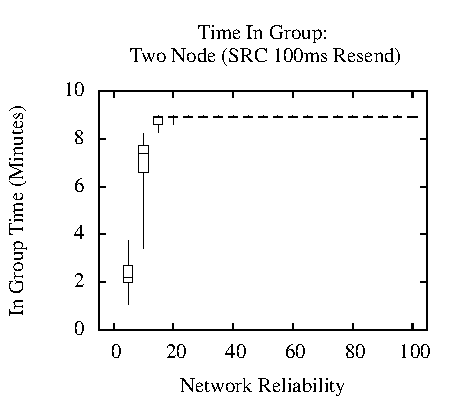
\includegraphics[width=\textwidth]{2NODE-SRC-100-GROUP.pdf}
    \caption{Time in-group over a 10 minute run for a two node system with a 100ms resend time}
    \label{fig:IGT-SRC-2NODE-100}
\end{minipage}%
\qquad
\begin{minipage}{0.45\textwidth}
    \centering
    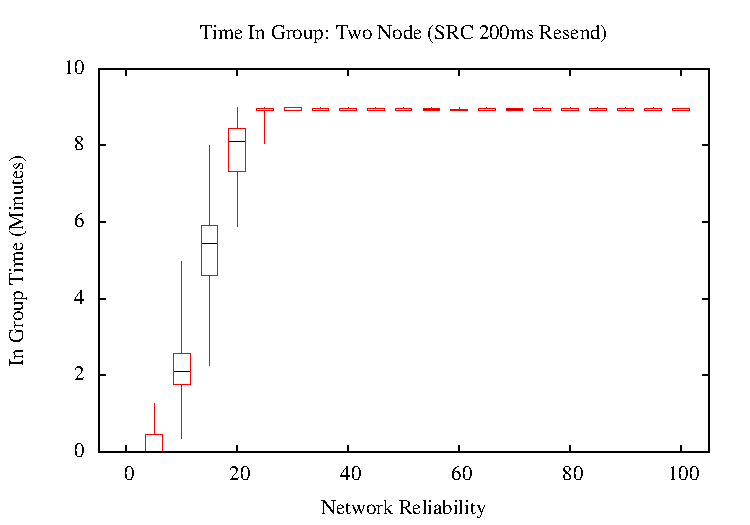
\includegraphics[width=\textwidth]{2NODE-SRC-200-GROUP.pdf}
    \caption{Time in-group over a 10 minute run for a two node system with a 200ms resend time}
    \label{fig:IGT-SRC-2NODE-200}
\end{minipage}
\end{figure}

The 100ms resend SRC test with two nodes can be considered a type of control in this study.
These tests, pictured in Figure \ref{fig:IGT-SRC-2NODE-100}, highlight the performance of the SRC protocol.
The maximum in group time of 9 minutes was achieved with only 15\% of datagrams arriving at the receiver. 

Figure \ref{fig:IGT-SRC-2NODE-200} demonstrates that as the rate at which lost datagrams were re-sent was decreased to 200ms, the in-group time decreased.
This behavior was expected.
Each exchange had a time limit for each message to arrive and the number of attempts was reduced by increasing the resend time.

\subsubsection{Transient Partition Case}

\begin{figure}
\centering
\begin{minipage}{0.45\textwidth}
    \centering
    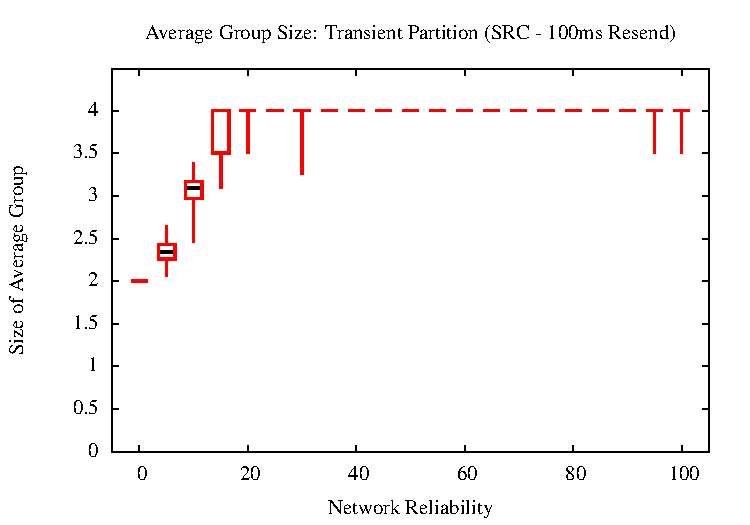
\includegraphics[width=\textwidth]{TRANS-SRC-100-SIZE.pdf}
    \caption{Average size of formed groups for the transient partition case with a 100ms resend time}
    \label{fig:MGS-SRC-TRANS-100}
\end{minipage}%
\qquad
\begin{minipage}{0.45\textwidth}
    \centering
    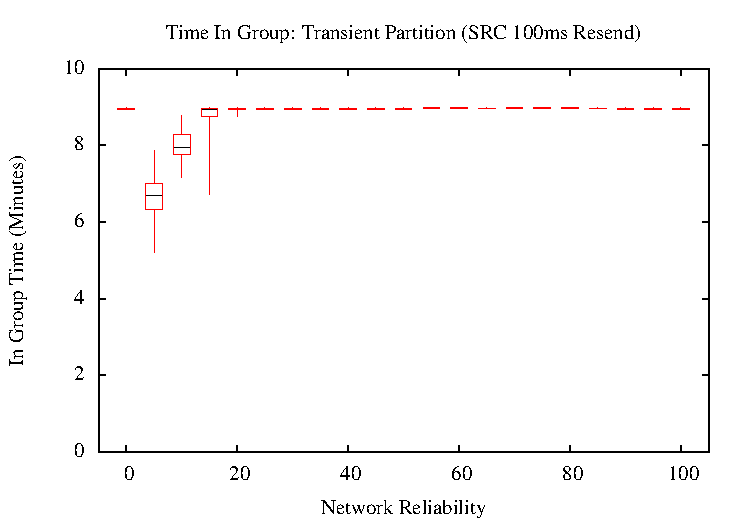
\includegraphics[width=\textwidth]{TRANS-SRC-100-GROUP.pdf}
    \caption{Time in-group over a 10 minute run for the transient partition case with a 100ms resend time}
    \label{fig:IGT-SRC-TRANS-100}
\end{minipage}
\end{figure}

The transient partition case is a simple example in which a network partition separates two groups of DGI processes. In the simplest case where the opposite side of the partition is unreachable, nodes will form a group with the other nodes on the same side of the partition.
In this study, two processes were present on each side of the partition.
In the experiment, the probability of a datagram crossing the partition was increased as the experiment continued.
The 100ms case is shown in Figures \ref{fig:MGS-SRC-TRANS-100} and \ref{fig:IGT-SRC-TRANS-100}.

While messages cannot cross the partition, the DGIs stay in a group with the nodes on the same side of the partition, leading to an in-group time of 9 minutes (the maximum value possible).
As packets began to cross the partition (as the omission rate decreases), DGI instances on either side attempted to complete elections with the nodes on the opposite partition and the in group time began to decrease.
During this time, however, the mean group size continued to increase.
Thus, while the elections were decreasing the amount of time that the module spent in a state where it can actively do work, it typically did not fall into a state where it was in a group by itself. 
As result, most of the lost in group time comes from elections.

\begin{figure}
\centering
\begin{minipage}{0.45\textwidth}
    \centering
    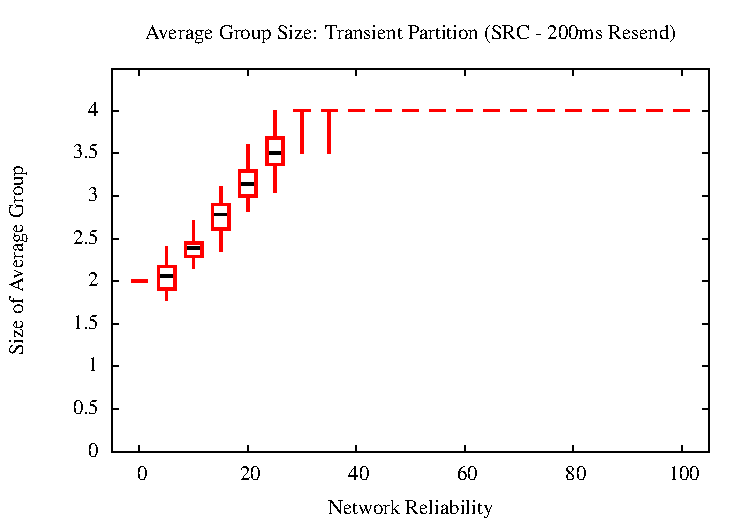
\includegraphics[width=\textwidth]{TRANS-SRC-200-SIZE.pdf}
    \caption{Average size of formed groups for the transient partition case with a 200ms resend time}
    \label{fig:MGS-SRC-TRANS-200}
\end{minipage}%
\qquad
\begin{minipage}{0.45\textwidth}
    \centering
    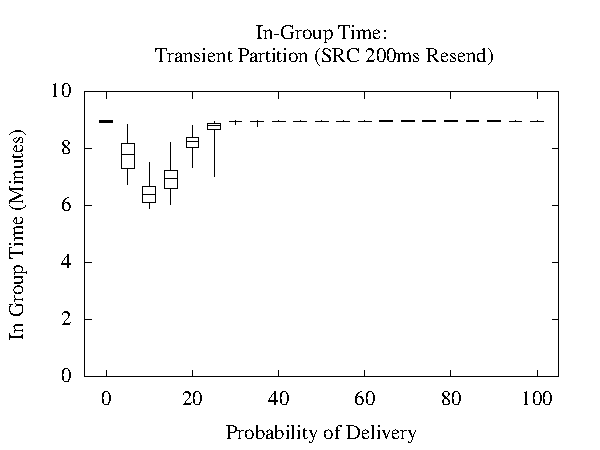
\includegraphics[width=\textwidth]{TRANS-SRC-200-GROUP.pdf}
    \caption{Time in-group over a 10 minute run for the transient partition case with a 200ms resend time}
    \label{fig:IGT-SRC-TRANS-200}
\end{minipage}
\end{figure}

The 200ms case (Illustrated in Figures \ref{fig:MGS-SRC-TRANS-200} and \ref{fig:IGT-SRC-TRANS-200}) suggests a similar behavior to Figures \ref{fig:MGS-SRC-TRANS-100} and \ref{fig:IGT-SRC-TRANS-100}, with a wider valley produced by the reduced number of datagrams.
The mean group size dips below 2 in Figure \ref{fig:MGS-SRC-TRANS-200}, possibly because longer resend times allowed for a greater number race conditions between potential leaders.
Discussion of these race conditions is shown and discussed during the SUC section since it was more prevalent in those experiments.

\subsection{Sequenced Unreliable Connection}

\subsubsection{Two Node Case}

The SUC protocol's experimental tests revealed an immediate problem.
There is a general increasing trend for the amount of time in-group shown in Figure \ref{fig:IGT-SUC-2NODE-100}.
There is a high amount of variance, however, for any particular trial.

\begin{figure}
\centering
\begin{minipage}{0.45\textwidth}
    \centering
    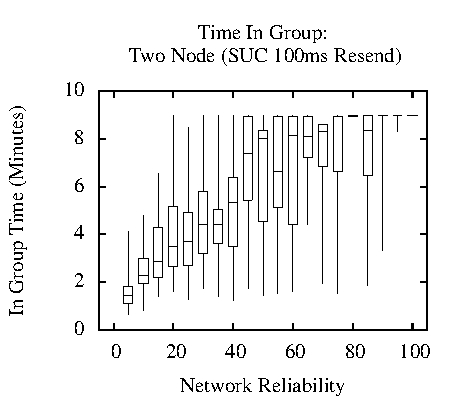
\includegraphics[width=\textwidth]{2NODE-SUC-100-GROUP.pdf}
    \caption{Time in group over a 10 minute run for two node system with 100ms resend time}
    \label{fig:IGT-SUC-2NODE-100}
\end{minipage}%
\qquad
\begin{minipage}{0.45\textwidth}
    \centering
    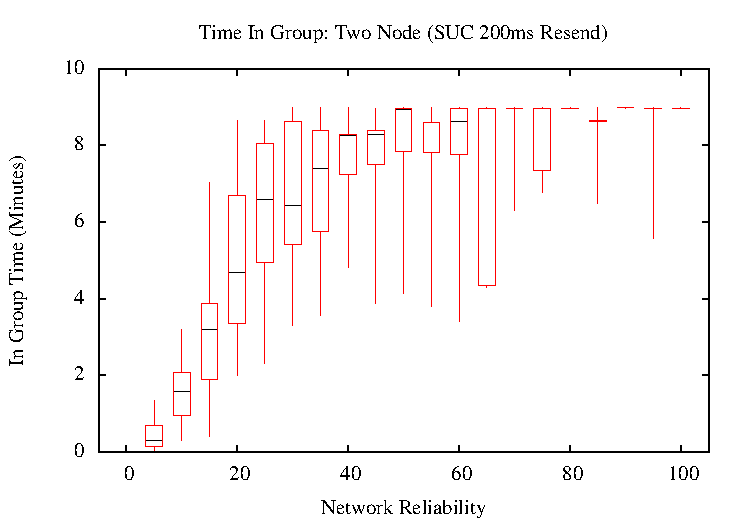
\includegraphics[width=\textwidth]{2NODE-SUC-200-GROUP.pdf}
    \caption{Time in group over a 10 minute run for two node system with 200ms resend time}
    \label{fig:IGT-SUC-2NODE-200}
\end{minipage}
\end{figure}

In the 200ms resend case (illustrated in Figure \ref{fig:IGT-SUC-2NODE-200}), a greater growth rate occurred in the in group time as the omission rate decreased.
When an average was taken across all of the collected data points from the experiment, the average in group time is higher for the 200ms case than it was for the 100ms case (6.86 vs 6.09).
There large amount of variance in the collected in group time, however.
As a result, it is not possible to state with confidence that the there is a significant difference between the two cases.


\section{Markov Models}

After collecting the results from the initial experiments, we sought to describe the observed behavior through the use of continuous-time Markov chains.
The behavior of the DGI transition between various states of grouping was calibrated with initial results and applied to other scenarios to validate the results.
This approach had several short comings.
First, for reasons we will demonstrate in subsequent chapters, the leader election algorithm modeled in these chains was not memoryless: the state used in the Markov chain was not sufficient capture the interaction between processes that was occurring.
Secondly, the continuous time model could not accurate capture the execution model of the DGI.
In the DGI processes synchronize with each-other to execute in a semi-synchronous manner.
As a result, the execution and transition between states is more accurately described with a discrete-time Markov chain.

\subsection{Initial Model Calibration}

The presented methodology of constructing the model was initially calibrated against the original two-node case.
This calibration used a non-real-time version of the DGI code.
The resulting Markov chain was processed using SharpE \cite{SHARPE}\cite{SHARPE2} made by Dr. Kishor Trivedi's group at Duke University, a popular tool for reliability analysis.
SharpE measured the reward collected in 600 seconds, minus the reward that was collected in the first 60 seconds. 
Discarding the reward from the first 60 seconds emulated the 60 seconds were discarded in the experimental runs.
The SharpE results are plotted along with the experimental results in Figures \ref{fig:COMPARE-SUC-2NODE-100} and \ref{fig:COMPARE-SUC-2NODE-200}.

\begin{figure}
\centering
\begin{minipage}{0.45\textwidth}
    \centering
    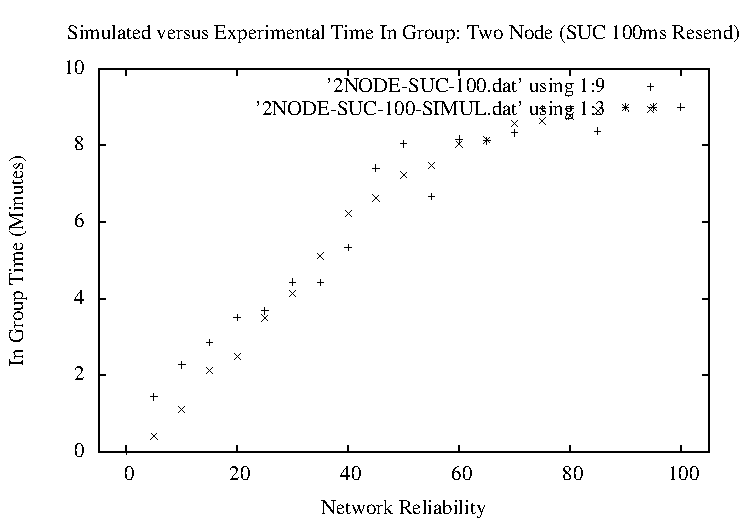
\includegraphics[width=1.0\textwidth]{2NODE-SUC-100-COMPARE.pdf}
    \caption{Comparison of in-group time as collected from the experimental platform and the simulator (1 tick offset between processes).}
    \label{fig:COMPARE-SUC-2NODE-100}
\end{minipage}%
\qquad
\begin{minipage}{0.45\textwidth}
    \centering
    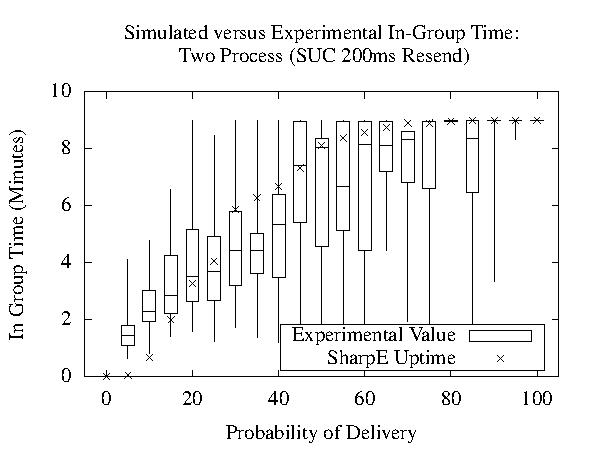
\includegraphics[width=1.0\textwidth]{2NODE-SUC-200-COMPARE.pdf}
    \caption{Comparison of in-group time as collected from the experimental platform and the simulator (2 tick offset between processes).}
    \label{fig:COMPARE-SUC-2NODE-200}
\end{minipage}
\end{figure}

The race condition between processes during an election is a consideration in the original leader election algorithm, and is an additional factor here.
The simulator provided a parameter to allow the operator to select how closely synchronized the peers were.
This synchronization was the time difference between when each of them would search for leaders.
The exchange of messages, particularly during an election, had a tendency to synchronize nodes during elections.
Nodes could synchronize even if they did not initially begin in a synchronized state. 
The simulation results aligned best for the 100ms resend case with 1 tick (Approximately 100ms difference in synchronization between processes) and 2 ticks (Approximately 400ms) in the 200ms resend case.

Models fit to the non-real-time code in groups larger than two processes had a poor fit.
This is presumed to be a combination of several factors.
The major source of fault included the structure of the chain. 
Construction of the chain assumes that all processes enter the election state a roughly the same time. 
This was not typically true for more than two processes.
Additionally, the simulator could only assume that the synchronization between processes was fixed.
The coincidental synchronization that occurred in the two node case was suppressed by the increased number of peers.
Furthermore, an issue with SharpE was discovered that prevented the particular structure of the chains produced from being handled correctly.
The election states with only one outbound transition uncovered a bug in the SharpE software.
To circumvent that, issue, SharpE was replaced by a random-walker which generates exponentially distributed numbers and follows the paths of the chain.
Time in group data for models which SharpE cannot process were collected across several hundred trials.

\begin{figure}
\centering
\begin{minipage}{0.45\textwidth}
    \centering
    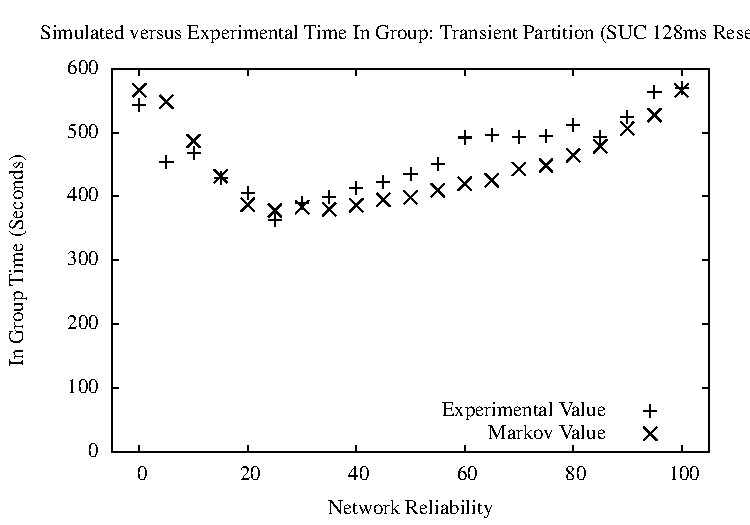
\includegraphics[width=1.0\textwidth]{TRANS-RT-SUC-128-COMPARE.pdf}
    \caption{Comparison of in-group time as collected from the experimental platform and the time in group from the equivalent Markov chain (128ms between resends).}
    \label{fig:COMPARE-SUC-TRANS-RT-128}
\end{minipage}%
\qquad
\begin{minipage}{0.45\textwidth}
    \centering
    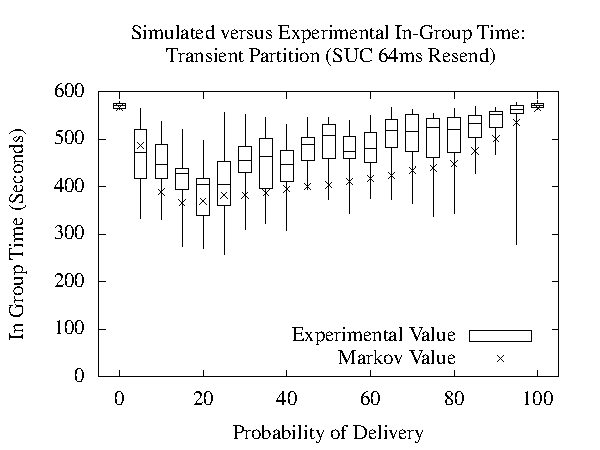
\includegraphics[width=1.0\textwidth]{TRANS-RT-SUC-64-COMPARE.pdf}
    \caption{Comparison of in-group time as collected from the experimental platform and the time in group from the equivalent Markov chain (64ms between resends).}
    \label{fig:COMPARE-SUC-TRANS-RT-64}
\end{minipage}
\end{figure}

The structure of the Markov Chain assumed that processes enter the election state simultaneously.
This was an appropriate assumption for the real-time system, since the round-robin scheduler synchronized when processes ran their group management modules.
The simulator was set to assume that the synchronization between processes was very tight.
New experimental data was collected for the 4 node, transient partition case.
The collected data is overlaid with the results from the random walker in Figures \ref{fig:COMPARE-SUC-TRANS-RT-128} and \ref{fig:COMPARE-SUC-TRANS-RT-64}.

\begin{table}
% increase table row spacing, adjust to taste
\caption{Error and correlation of experimental data and Markov chain predictions}
\label{tab:STAT-DATA}
\centering
% Some packages, such as MDW tools, offer better commands for making tables
% than the plain LaTeX2e tabular which is used here.
\begin{tabular}{|c||c|c|c|}
\hline
Re-send & Correlation & Error \\ \hline
128 & 0.7656 & 11.61\% \\ \hline
64 & 0.8604 & 11.70\% \\ \hline
\end{tabular}
\end{table}

As a measure of the strength of the model, the correlation between the predicted value was compared.
The average error was also computed for each of the samples taken.
This information is presented in Table \ref{tab:STAT-DATA}.
These results results were not sufficient to accurately describe the behavior of the system during fault conditions.
As a result, we sought to refine the analysis of the model in order to get an accurate portrayal of the behavior of the system during faults.

\section{Remarks}

In order to ensure that critical infrastructure safely and reliably provides services to those that need the services, it is necessary to understand how the infrastructure behaves during faults.
Conceptually, using unvetted critical infrastructure, especially when the infrastructure relies heavily on communication, is the same as stepping into an elevator without a safety brake.
Strong analysis of a system's behavior during a failure scenario is paramount to ensuring the safety of those using the infrastructure.
We propose knowledge of the correctness of the operation may be more important that the efficiency of the operation of that critical infrastructure.
Through this work we demonstrate how distributed algorithms can be improved by reasoning about them using information flow security models.
By using these models one can analyze where the certainty of the system is placed, as well as ensuring that the algorithms can be modeled without complete and perfect information of the system.

Additionally, we wish to show that these models can be used to allow the models to go beyond use by those administrating the infrastructure.
The models created can be analyzed and used while the system is working to provide services (``online'').
Using the models created in this way a distributed critical infrastructure system can adjust it behavior, hardening itself against failures that could arise.
With this hardening technique the algorithms can prevent critical failures which could decrease quality of life or endanger that life itself.
Subsequent chapters show how information flow methods can be used to determine the memorylessness of aspects of a distributed system, how those aspects can be used to construct a model, and applications of those models.
